% Options for packages loaded elsewhere
\PassOptionsToPackage{unicode}{hyperref}
\PassOptionsToPackage{hyphens}{url}
%
\documentclass[
]{article}
\usepackage{amsmath,amssymb}
\usepackage{iftex}
\ifPDFTeX
  \usepackage[T1]{fontenc}
  \usepackage[utf8]{inputenc}
  \usepackage{textcomp} % provide euro and other symbols
\else % if luatex or xetex
  \usepackage{unicode-math} % this also loads fontspec
  \defaultfontfeatures{Scale=MatchLowercase}
  \defaultfontfeatures[\rmfamily]{Ligatures=TeX,Scale=1}
\fi
\usepackage{lmodern}
\ifPDFTeX\else
  % xetex/luatex font selection
    \setmainfont[]{YuGothic}
\fi
% Use upquote if available, for straight quotes in verbatim environments
\IfFileExists{upquote.sty}{\usepackage{upquote}}{}
\IfFileExists{microtype.sty}{% use microtype if available
  \usepackage[]{microtype}
  \UseMicrotypeSet[protrusion]{basicmath} % disable protrusion for tt fonts
}{}
\makeatletter
\@ifundefined{KOMAClassName}{% if non-KOMA class
  \IfFileExists{parskip.sty}{%
    \usepackage{parskip}
  }{% else
    \setlength{\parindent}{0pt}
    \setlength{\parskip}{6pt plus 2pt minus 1pt}}
}{% if KOMA class
  \KOMAoptions{parskip=half}}
\makeatother
\usepackage{xcolor}
\usepackage[margin=1in]{geometry}
\usepackage{color}
\usepackage{fancyvrb}
\newcommand{\VerbBar}{|}
\newcommand{\VERB}{\Verb[commandchars=\\\{\}]}
\DefineVerbatimEnvironment{Highlighting}{Verbatim}{commandchars=\\\{\}}
% Add ',fontsize=\small' for more characters per line
\usepackage{framed}
\definecolor{shadecolor}{RGB}{248,248,248}
\newenvironment{Shaded}{\begin{snugshade}}{\end{snugshade}}
\newcommand{\AlertTok}[1]{\textcolor[rgb]{0.94,0.16,0.16}{#1}}
\newcommand{\AnnotationTok}[1]{\textcolor[rgb]{0.56,0.35,0.01}{\textbf{\textit{#1}}}}
\newcommand{\AttributeTok}[1]{\textcolor[rgb]{0.13,0.29,0.53}{#1}}
\newcommand{\BaseNTok}[1]{\textcolor[rgb]{0.00,0.00,0.81}{#1}}
\newcommand{\BuiltInTok}[1]{#1}
\newcommand{\CharTok}[1]{\textcolor[rgb]{0.31,0.60,0.02}{#1}}
\newcommand{\CommentTok}[1]{\textcolor[rgb]{0.56,0.35,0.01}{\textit{#1}}}
\newcommand{\CommentVarTok}[1]{\textcolor[rgb]{0.56,0.35,0.01}{\textbf{\textit{#1}}}}
\newcommand{\ConstantTok}[1]{\textcolor[rgb]{0.56,0.35,0.01}{#1}}
\newcommand{\ControlFlowTok}[1]{\textcolor[rgb]{0.13,0.29,0.53}{\textbf{#1}}}
\newcommand{\DataTypeTok}[1]{\textcolor[rgb]{0.13,0.29,0.53}{#1}}
\newcommand{\DecValTok}[1]{\textcolor[rgb]{0.00,0.00,0.81}{#1}}
\newcommand{\DocumentationTok}[1]{\textcolor[rgb]{0.56,0.35,0.01}{\textbf{\textit{#1}}}}
\newcommand{\ErrorTok}[1]{\textcolor[rgb]{0.64,0.00,0.00}{\textbf{#1}}}
\newcommand{\ExtensionTok}[1]{#1}
\newcommand{\FloatTok}[1]{\textcolor[rgb]{0.00,0.00,0.81}{#1}}
\newcommand{\FunctionTok}[1]{\textcolor[rgb]{0.13,0.29,0.53}{\textbf{#1}}}
\newcommand{\ImportTok}[1]{#1}
\newcommand{\InformationTok}[1]{\textcolor[rgb]{0.56,0.35,0.01}{\textbf{\textit{#1}}}}
\newcommand{\KeywordTok}[1]{\textcolor[rgb]{0.13,0.29,0.53}{\textbf{#1}}}
\newcommand{\NormalTok}[1]{#1}
\newcommand{\OperatorTok}[1]{\textcolor[rgb]{0.81,0.36,0.00}{\textbf{#1}}}
\newcommand{\OtherTok}[1]{\textcolor[rgb]{0.56,0.35,0.01}{#1}}
\newcommand{\PreprocessorTok}[1]{\textcolor[rgb]{0.56,0.35,0.01}{\textit{#1}}}
\newcommand{\RegionMarkerTok}[1]{#1}
\newcommand{\SpecialCharTok}[1]{\textcolor[rgb]{0.81,0.36,0.00}{\textbf{#1}}}
\newcommand{\SpecialStringTok}[1]{\textcolor[rgb]{0.31,0.60,0.02}{#1}}
\newcommand{\StringTok}[1]{\textcolor[rgb]{0.31,0.60,0.02}{#1}}
\newcommand{\VariableTok}[1]{\textcolor[rgb]{0.00,0.00,0.00}{#1}}
\newcommand{\VerbatimStringTok}[1]{\textcolor[rgb]{0.31,0.60,0.02}{#1}}
\newcommand{\WarningTok}[1]{\textcolor[rgb]{0.56,0.35,0.01}{\textbf{\textit{#1}}}}
\usepackage{longtable,booktabs,array}
\usepackage{calc} % for calculating minipage widths
% Correct order of tables after \paragraph or \subparagraph
\usepackage{etoolbox}
\makeatletter
\patchcmd\longtable{\par}{\if@noskipsec\mbox{}\fi\par}{}{}
\makeatother
% Allow footnotes in longtable head/foot
\IfFileExists{footnotehyper.sty}{\usepackage{footnotehyper}}{\usepackage{footnote}}
\makesavenoteenv{longtable}
\usepackage{graphicx}
\makeatletter
\newsavebox\pandoc@box
\newcommand*\pandocbounded[1]{% scales image to fit in text height/width
  \sbox\pandoc@box{#1}%
  \Gscale@div\@tempa{\textheight}{\dimexpr\ht\pandoc@box+\dp\pandoc@box\relax}%
  \Gscale@div\@tempb{\linewidth}{\wd\pandoc@box}%
  \ifdim\@tempb\p@<\@tempa\p@\let\@tempa\@tempb\fi% select the smaller of both
  \ifdim\@tempa\p@<\p@\scalebox{\@tempa}{\usebox\pandoc@box}%
  \else\usebox{\pandoc@box}%
  \fi%
}
% Set default figure placement to htbp
\def\fps@figure{htbp}
\makeatother
\setlength{\emergencystretch}{3em} % prevent overfull lines
\providecommand{\tightlist}{%
  \setlength{\itemsep}{0pt}\setlength{\parskip}{0pt}}
\setcounter{secnumdepth}{5}
\usepackage{zxjatype}
\setjamainfont{YuGothic}
\parindent=0pt
\parskip=6pt
\renewcommand{\baselinestretch}{1.2}
\tolerance=1000
\pretolerance=1000
\sloppy
\usepackage{float}
\usepackage{booktabs}
\usepackage{longtable}
\usepackage{array}
\usepackage{multirow}
\usepackage{wrapfig}
\usepackage{colortbl}
\usepackage{pdflscape}
\usepackage{tabu}
\usepackage{threeparttable}
\usepackage{threeparttablex}
\usepackage[normalem]{ulem}
\usepackage{makecell}
\usepackage{xcolor}
\usepackage{bookmark}
\IfFileExists{xurl.sty}{\usepackage{xurl}}{} % add URL line breaks if available
\urlstyle{same}
\hypersetup{
  pdftitle={note記事アクセス分析レポート},
  pdfauthor={Masahito},
  hidelinks,
  pdfcreator={LaTeX via pandoc}}

\title{note記事アクセス分析レポート}
\author{Masahito}
\date{2025-06-29}

\begin{document}
\maketitle

{
\setcounter{tocdepth}{2}
\tableofcontents
}
\section{はじめに}\label{ux306fux3058ux3081ux306b}

このレポートでは、仮想note記事データをもとに、どんな条件の記事がより多く読まれるのか分析・可視化し、傾向を把握します。
さらに、閲覧された記事のエンゲージメント(ユーザーの反応:スキ)について詳しく分析します。

\begin{center}\rule{0.5\linewidth}{0.5pt}\end{center}

\section{データ内容の確認}\label{ux30c7ux30fcux30bfux5185ux5bb9ux306eux78baux8a8d}

\begin{Shaded}
\begin{Highlighting}[]
\DocumentationTok{\#\#データの読み込み}
\NormalTok{note\_data }\OtherTok{\textless{}{-}} \FunctionTok{read\_csv}\NormalTok{(}\StringTok{"step01\_note\_virtual\_data.csv"}\NormalTok{)}
\DocumentationTok{\#\#データの構造確認}
\NormalTok{glimpse\_text }\OtherTok{\textless{}{-}} \FunctionTok{capture.output}\NormalTok{(}\FunctionTok{glimpse}\NormalTok{(note\_data))}
\FunctionTok{cat}\NormalTok{(}\FunctionTok{paste}\NormalTok{(glimpse\_text, }\AttributeTok{collapse =} \StringTok{"}\SpecialCharTok{\textbackslash{}n}\StringTok{"}\NormalTok{))}
\end{Highlighting}
\end{Shaded}

Rows: 15 Columns: 6 \$ title ``AI時代に必要なスキルとは'',
``30代でキャリアに悩んだときに読んだ本'', ``SNS疲れから抜け出す方法'',
``副業を始め\textasciitilde{} \$ length 2051, 1716, 2455, 2186, 1881,
1938, 1345, 2368, 1785, 2210, 197\textasciitilde{} \$ time 10:37:00,
18:11:00, 23:50:00, 05:20:00, 14:27:00, 13:14:00, 20\textasciitilde{} \$
tag ''キャリア,働き方'', ``読書,ライフハック'', ``SNS,メンタル'',
``副業,マネー'', ``生活習慣,朝活'', ``健康,ラ\textasciitilde{} \$ pv
1233, 1289, 833, 636, 1122, 1171, 664, 789, 1142, 1256, 351,
76\textasciitilde{} \$ likes 79, 123, 47, 61, 72, 123, 53, 143, 185, 98,
48, 139, 64, 196, 49

\begin{Shaded}
\begin{Highlighting}[]
\DocumentationTok{\#\#各数値の要約}
\FunctionTok{summary}\NormalTok{(note\_data)}
\end{Highlighting}
\end{Shaded}

\begin{verbatim}
title               length          time              tag           
\end{verbatim}

Length:15 Min. :1274 Min. :01:31:00 Length:15\\
Class :character 1st Qu.:1750 1st Qu.:07:26:00 Class :character\\
Mode :character Median :1948 Median :10:37:00 Mode :character\\
Mean :1897 Mean :12:33:40\\
3rd Qu.:2118 3rd Qu.:19:17:00\\
Max. :2455 Max. :23:50:00\\
pv likes\\
Min. : 351.0 Min. : 47.00\\
1st Qu.: 716.0 1st Qu.: 57.00\\
Median :1122.0 Median : 79.00\\
Mean : 949.3 Mean : 98.67\\
3rd Qu.:1207.5 3rd Qu.:131.00\\
Max. :1369.0 Max. :196.00

\begin{Shaded}
\begin{Highlighting}[]
\DocumentationTok{\#\#欠損値の有無}
\FunctionTok{colSums}\NormalTok{(}\FunctionTok{is.na}\NormalTok{(note\_data))}
\end{Highlighting}
\end{Shaded}

title length time tag pv likes 0 0 0 0 0 0

\begin{center}\rule{0.5\linewidth}{0.5pt}\end{center}

\section{データの前処理}\label{ux30c7ux30fcux30bfux306eux524dux51e6ux7406}

\begin{Shaded}
\begin{Highlighting}[]
\DocumentationTok{\#\#タイトル文字数}
\NormalTok{note\_data }\OtherTok{\textless{}{-}}\NormalTok{ note\_data }\SpecialCharTok{\%\textgreater{}\%}
  \FunctionTok{mutate}\NormalTok{(}\AttributeTok{title\_num =} \FunctionTok{nchar}\NormalTok{(title))}
\DocumentationTok{\#\#スキ率列の追加}
\NormalTok{note\_data }\OtherTok{\textless{}{-}}\NormalTok{ note\_data }\SpecialCharTok{\%\textgreater{}\%}
  \FunctionTok{mutate}\NormalTok{(}\AttributeTok{like\_rate =}\NormalTok{ likes }\SpecialCharTok{/}\NormalTok{ pv)}
\DocumentationTok{\#\#タグの分解}
\NormalTok{note\_data\_long }\OtherTok{\textless{}{-}}\NormalTok{ note\_data }\SpecialCharTok{\%\textgreater{}\%}
  \FunctionTok{separate\_rows}\NormalTok{(tag, }\AttributeTok{sep =} \StringTok{",}\SpecialCharTok{\textbackslash{}\textbackslash{}}\StringTok{s*"}\NormalTok{) }\SpecialCharTok{\%\textgreater{}\%}
  \FunctionTok{mutate}\NormalTok{(}\AttributeTok{tag =} \FunctionTok{str\_trim}\NormalTok{(tag))}
\DocumentationTok{\#\#タグの重複チェック}
\NormalTok{note\_data\_long }\SpecialCharTok{\%\textgreater{}\%}
  \FunctionTok{count}\NormalTok{(tag) }\SpecialCharTok{\%\textgreater{}\%}
  \FunctionTok{arrange}\NormalTok{(}\FunctionTok{desc}\NormalTok{(n))}
\end{Highlighting}
\end{Shaded}

\begin{verbatim}
## # A tibble: 29 x 2
##    tag              n
##    <chr>        <int>
##  1 読書             2
##  2 AI               1
##  3 SNS              1
##  4 Z世代            1
##  5 note             1
##  6 アクセス解析     1
##  7 キャリア         1
##  8 デザイン         1
##  9 ブログ           1
## 10 マネー           1
## # i 19 more rows
\end{verbatim}

\begin{Shaded}
\begin{Highlighting}[]
\DocumentationTok{\#\#時間帯カテゴリの追加}
\NormalTok{note\_data }\OtherTok{\textless{}{-}}\NormalTok{ note\_data }\SpecialCharTok{\%\textgreater{}\%}
  \FunctionTok{mutate}\NormalTok{(}
    \AttributeTok{time\_hms =}\NormalTok{ hms}\SpecialCharTok{::}\FunctionTok{as\_hms}\NormalTok{(}\FunctionTok{paste0}\NormalTok{(time, }\StringTok{":00"}\NormalTok{)),}
    \AttributeTok{time\_hours =} \FunctionTok{hour}\NormalTok{(time\_hms) }\SpecialCharTok{+} \FunctionTok{minute}\NormalTok{(time\_hms)}\SpecialCharTok{/}\DecValTok{60}
\NormalTok{  )}
\NormalTok{note\_data }\OtherTok{\textless{}{-}}\NormalTok{ note\_data }\SpecialCharTok{\%\textgreater{}\%}
  \FunctionTok{mutate}\NormalTok{(}\AttributeTok{time\_category =} \FunctionTok{case\_when}\NormalTok{(}
\NormalTok{    time\_hours }\SpecialCharTok{\textless{}} \DecValTok{12} \SpecialCharTok{\textasciitilde{}} \StringTok{"朝"}\NormalTok{,}
\NormalTok{    time\_hours }\SpecialCharTok{\textless{}} \DecValTok{18} \SpecialCharTok{\textasciitilde{}} \StringTok{"昼"}\NormalTok{,}
    \ConstantTok{TRUE} \SpecialCharTok{\textasciitilde{}} \StringTok{"夜"}
\NormalTok{  ))}
\DocumentationTok{\#\#文字数カテゴリの追加}
\NormalTok{note\_data }\OtherTok{\textless{}{-}}\NormalTok{ note\_data }\SpecialCharTok{\%\textgreater{}\%}
  \FunctionTok{mutate}\NormalTok{(}\AttributeTok{length\_category =} \FunctionTok{case\_when}\NormalTok{(}
\NormalTok{    length }\SpecialCharTok{\textless{}} \DecValTok{800} \SpecialCharTok{\textasciitilde{}} \StringTok{"短文"}\NormalTok{,}
\NormalTok{    length }\SpecialCharTok{\textless{}} \DecValTok{1500} \SpecialCharTok{\textasciitilde{}} \StringTok{"中文"}\NormalTok{,}
    \ConstantTok{TRUE} \SpecialCharTok{\textasciitilde{}} \StringTok{"長文"}
\NormalTok{  ))}
\DocumentationTok{\#\#文字数カテゴリの可視化}
\FunctionTok{showtext\_auto}\NormalTok{()}
\end{Highlighting}
\end{Shaded}

\begin{center}\rule{0.5\linewidth}{0.5pt}\end{center}

\section{データ解析(閲覧数)}\label{ux30c7ux30fcux30bfux89e3ux6790ux95b2ux89a7ux6570}

\begin{Shaded}
\begin{Highlighting}[]
\DocumentationTok{\#\#タイトルの文字数と閲覧数の関係}
\FunctionTok{ggplot}\NormalTok{(note\_data, }\FunctionTok{aes}\NormalTok{(}\AttributeTok{x =}\NormalTok{ title\_num, }\AttributeTok{y =}\NormalTok{ pv)) }\SpecialCharTok{+}
  \FunctionTok{geom\_point}\NormalTok{() }\SpecialCharTok{+}
  \FunctionTok{geom\_smooth}\NormalTok{(}\AttributeTok{method =} \StringTok{"lm"}\NormalTok{, }\AttributeTok{se =} \ConstantTok{FALSE}\NormalTok{) }\SpecialCharTok{+}
  \FunctionTok{labs}\NormalTok{(}\AttributeTok{title =} \StringTok{"タイトル文字数と閲覧数の関係"}\NormalTok{, }\AttributeTok{x =} \StringTok{"文字数"}\NormalTok{, }\AttributeTok{y =} \StringTok{"閲覧数"}\NormalTok{)}
\end{Highlighting}
\end{Shaded}

\pandocbounded{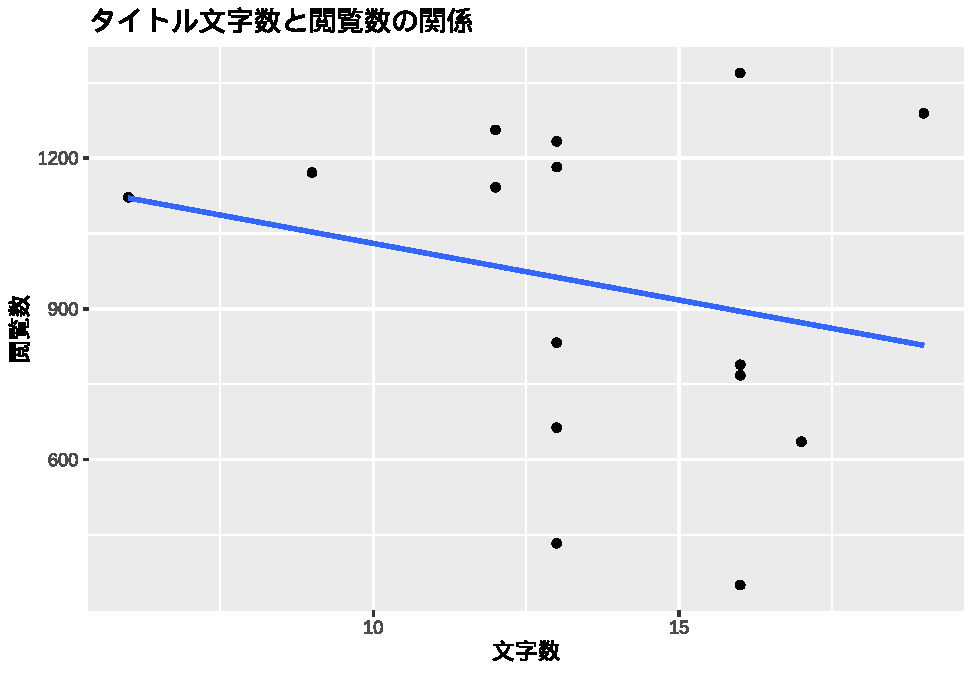
\includegraphics[keepaspectratio]{note-report_files/figure-latex/unnamed-chunk-2-1.pdf}}

\begin{Shaded}
\begin{Highlighting}[]
\DocumentationTok{\#\#投稿時間と閲覧数の関係}
\FunctionTok{ggplot}\NormalTok{(note\_data, }\FunctionTok{aes}\NormalTok{(}\AttributeTok{x =}\NormalTok{ time, }\AttributeTok{y =}\NormalTok{ pv)) }\SpecialCharTok{+}
  \FunctionTok{geom\_point}\NormalTok{() }\SpecialCharTok{+}
  \FunctionTok{geom\_smooth}\NormalTok{(}\AttributeTok{method =} \StringTok{"lm"}\NormalTok{, }\AttributeTok{se =} \ConstantTok{FALSE}\NormalTok{) }\SpecialCharTok{+}
  \FunctionTok{labs}\NormalTok{(}\AttributeTok{title =} \StringTok{"投稿時間と閲覧数の関係"}\NormalTok{, }\AttributeTok{x =} \StringTok{"投稿時間"}\NormalTok{, }\AttributeTok{y =} \StringTok{"閲覧数"}\NormalTok{)}
\end{Highlighting}
\end{Shaded}

\pandocbounded{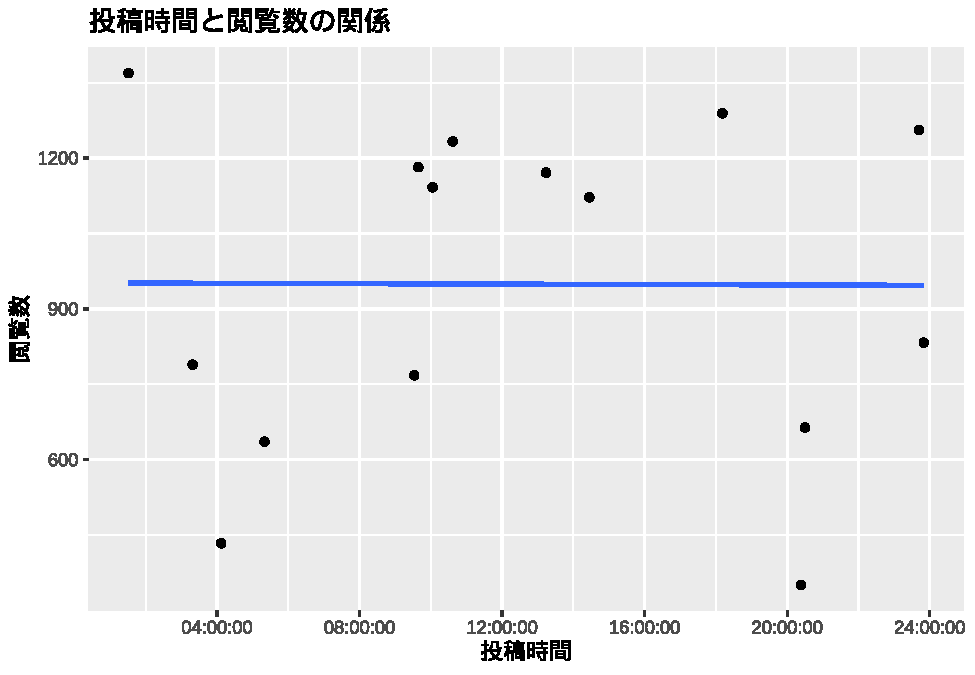
\includegraphics[keepaspectratio]{note-report_files/figure-latex/unnamed-chunk-2-2.pdf}}

\begin{Shaded}
\begin{Highlighting}[]
\DocumentationTok{\#\#投稿時間帯と閲覧数の関係}
\NormalTok{note\_data }\OtherTok{\textless{}{-}}\NormalTok{ note\_data }\SpecialCharTok{\%\textgreater{}\%}
  \FunctionTok{mutate}\NormalTok{(}\AttributeTok{time\_category =} \FunctionTok{factor}\NormalTok{(time\_category, }\AttributeTok{levels =} \FunctionTok{c}\NormalTok{(}\StringTok{"朝"}\NormalTok{, }\StringTok{"昼"}\NormalTok{, }\StringTok{"夜"}\NormalTok{)))}
\FunctionTok{ggplot}\NormalTok{(note\_data, }\FunctionTok{aes}\NormalTok{(}\AttributeTok{x =}\NormalTok{ time\_category, }\AttributeTok{y =}\NormalTok{ pv)) }\SpecialCharTok{+}
  \FunctionTok{geom\_boxplot}\NormalTok{() }\SpecialCharTok{+}
  \FunctionTok{labs}\NormalTok{(}\AttributeTok{title =} \StringTok{"時間帯別の閲覧数(PV)"}\NormalTok{, }\AttributeTok{x =} \StringTok{"時間帯"}\NormalTok{, }\AttributeTok{y =} \StringTok{"閲覧数"}\NormalTok{)}
\end{Highlighting}
\end{Shaded}

\pandocbounded{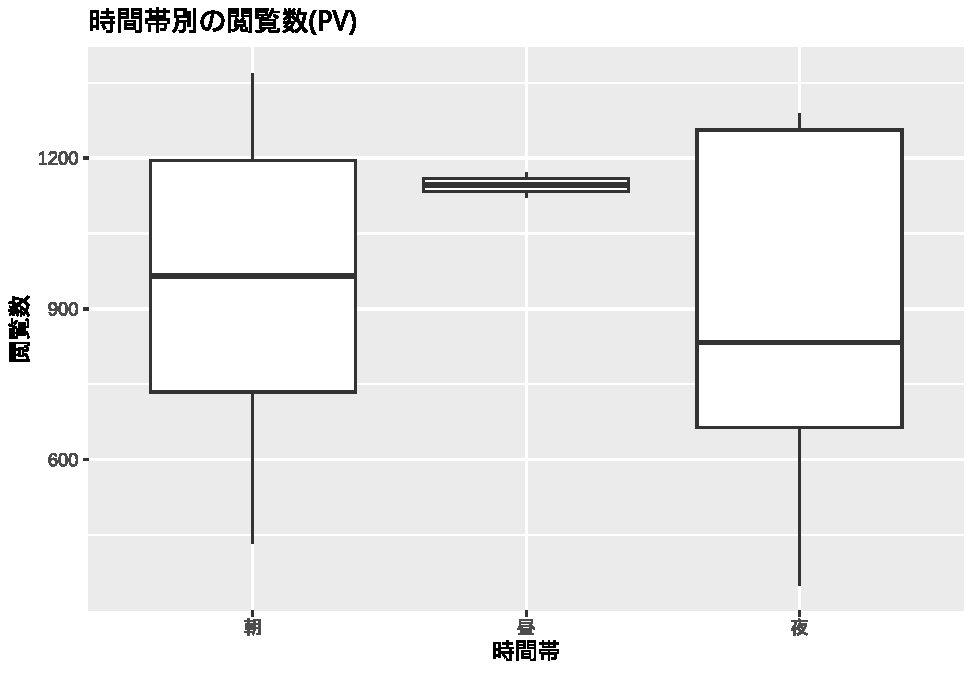
\includegraphics[keepaspectratio]{note-report_files/figure-latex/unnamed-chunk-2-3.pdf}}

\begin{Shaded}
\begin{Highlighting}[]
\DocumentationTok{\#\#文字数と閲覧数の関係}
\FunctionTok{ggplot}\NormalTok{(note\_data, }\FunctionTok{aes}\NormalTok{(}\AttributeTok{x =}\NormalTok{ length, }\AttributeTok{y =}\NormalTok{ pv)) }\SpecialCharTok{+}
  \FunctionTok{geom\_point}\NormalTok{() }\SpecialCharTok{+}
  \FunctionTok{geom\_smooth}\NormalTok{(}\AttributeTok{method =} \StringTok{"lm"}\NormalTok{, }\AttributeTok{se =} \ConstantTok{FALSE}\NormalTok{) }\SpecialCharTok{+}
  \FunctionTok{labs}\NormalTok{(}\AttributeTok{title =} \StringTok{"文字数と閲覧数の関係"}\NormalTok{, }\AttributeTok{x =} \StringTok{"文字数"}\NormalTok{, }\AttributeTok{y =} \StringTok{"閲覧数"}\NormalTok{)}
\end{Highlighting}
\end{Shaded}

\pandocbounded{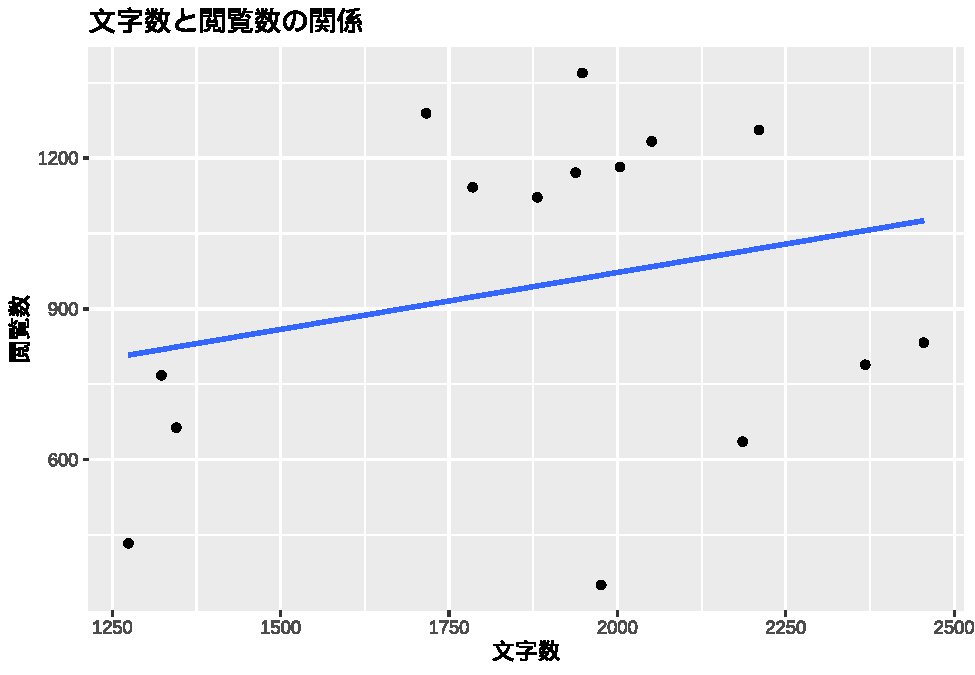
\includegraphics[keepaspectratio]{note-report_files/figure-latex/unnamed-chunk-2-4.pdf}}

\begin{Shaded}
\begin{Highlighting}[]
\DocumentationTok{\#\#タグ別の平均閲覧数}
\NormalTok{note\_data }\SpecialCharTok{\%\textgreater{}\%}
  \FunctionTok{summarise}\NormalTok{(}
    \AttributeTok{avg\_pv =} \FunctionTok{mean}\NormalTok{(pv)}
\NormalTok{  )}
\end{Highlighting}
\end{Shaded}

\begin{verbatim}
## # A tibble: 1 x 1
##   avg_pv
##    <dbl>
## 1   949.
\end{verbatim}

\begin{Shaded}
\begin{Highlighting}[]
\NormalTok{tag\_summary }\OtherTok{\textless{}{-}}\NormalTok{ note\_data\_long }\SpecialCharTok{\%\textgreater{}\%}
  \FunctionTok{group\_by}\NormalTok{(tag) }\SpecialCharTok{\%\textgreater{}\%}
  \FunctionTok{summarise}\NormalTok{(}\AttributeTok{mean\_pv =} \FunctionTok{mean}\NormalTok{(pv), }\AttributeTok{.groups =} \StringTok{"drop"}\NormalTok{)}
\FunctionTok{ggplot}\NormalTok{(tag\_summary, }\FunctionTok{aes}\NormalTok{(}\AttributeTok{x =} \FunctionTok{reorder}\NormalTok{(tag, mean\_pv), }\AttributeTok{y =}\NormalTok{ mean\_pv)) }\SpecialCharTok{+}
  \FunctionTok{geom\_col}\NormalTok{() }\SpecialCharTok{+}
  \FunctionTok{coord\_flip}\NormalTok{() }\SpecialCharTok{+}
  \FunctionTok{labs}\NormalTok{(}\AttributeTok{title =} \StringTok{"タグ別平均閲覧数"}\NormalTok{, }\AttributeTok{x =} \StringTok{"タグ"}\NormalTok{, }\AttributeTok{y =} \StringTok{"平均閲覧数"}\NormalTok{)}
\end{Highlighting}
\end{Shaded}

\pandocbounded{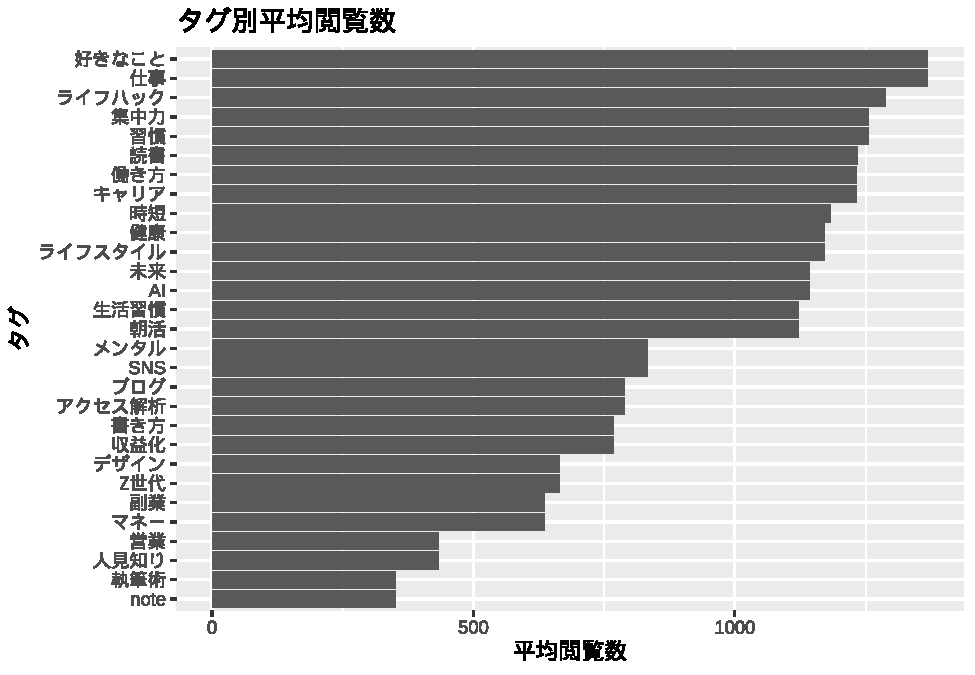
\includegraphics[keepaspectratio]{note-report_files/figure-latex/unnamed-chunk-2-5.pdf}}

\begin{Shaded}
\begin{Highlighting}[]
\DocumentationTok{\#\#閲覧数が高い記事の特徴を見る}
\NormalTok{note\_data }\SpecialCharTok{\%\textgreater{}\%}
  \FunctionTok{arrange}\NormalTok{(}\FunctionTok{desc}\NormalTok{(pv)) }\SpecialCharTok{\%\textgreater{}\%}
  \FunctionTok{select}\NormalTok{(title, title\_num, time, length, pv, likes, like\_rate) }\SpecialCharTok{\%\textgreater{}\%}
  \FunctionTok{head}\NormalTok{(}\DecValTok{5}\NormalTok{)}
\end{Highlighting}
\end{Shaded}

\begin{verbatim}
## # A tibble: 5 x 7
##   title                             title_num time  length    pv likes like_rate
##   <chr>                                 <int> <tim>  <dbl> <dbl> <dbl>     <dbl>
## 1 「好き」を仕事にするための第一歩         16 01:31   1948  1369   196    0.143 
## 2 30代でキャリアに悩んだときに読んだ本~~        19 18:11   1716  1289   123    0.0954
## 3 集中力を高める3つの習慣                  12 23:42   2210  1256    98    0.0780
## 4 AI時代に必要なスキルとは                 13 10:37   2051  1233    79    0.0641
## 5 忙しい人のための時短読書術               13 09:39   2004  1182    64    0.0541
\end{verbatim}

\begin{center}\rule{0.5\linewidth}{0.5pt}\end{center}

\section{データ解析(エンゲージメント:スキ数)}\label{ux30c7ux30fcux30bfux89e3ux6790ux30a8ux30f3ux30b2ux30fcux30b8ux30e1ux30f3ux30c8ux30b9ux30adux6570}

\begin{Shaded}
\begin{Highlighting}[]
\DocumentationTok{\#\#閲覧数とスキ数との相関関係}
\FunctionTok{cor}\NormalTok{(note\_data}\SpecialCharTok{$}\NormalTok{pv, note\_data}\SpecialCharTok{$}\NormalTok{likes)}
\end{Highlighting}
\end{Shaded}

\begin{verbatim}
## [1] 0.5419124
\end{verbatim}

\begin{Shaded}
\begin{Highlighting}[]
\DocumentationTok{\#\#タイトルの文字数とスキ数の関係}
\FunctionTok{ggplot}\NormalTok{(note\_data, }\FunctionTok{aes}\NormalTok{(}\AttributeTok{x =}\NormalTok{ title\_num, }\AttributeTok{y =}\NormalTok{ likes)) }\SpecialCharTok{+}
  \FunctionTok{geom\_point}\NormalTok{() }\SpecialCharTok{+}
  \FunctionTok{geom\_smooth}\NormalTok{(}\AttributeTok{method =} \StringTok{"lm"}\NormalTok{, }\AttributeTok{se =} \ConstantTok{FALSE}\NormalTok{) }\SpecialCharTok{+}
  \FunctionTok{labs}\NormalTok{(}\AttributeTok{title =} \StringTok{"タイトル文字数とスキ数の関係"}\NormalTok{, }\AttributeTok{x =} \StringTok{"文字数"}\NormalTok{, }\AttributeTok{y =} \StringTok{"スキ数"}\NormalTok{)}
\end{Highlighting}
\end{Shaded}

\pandocbounded{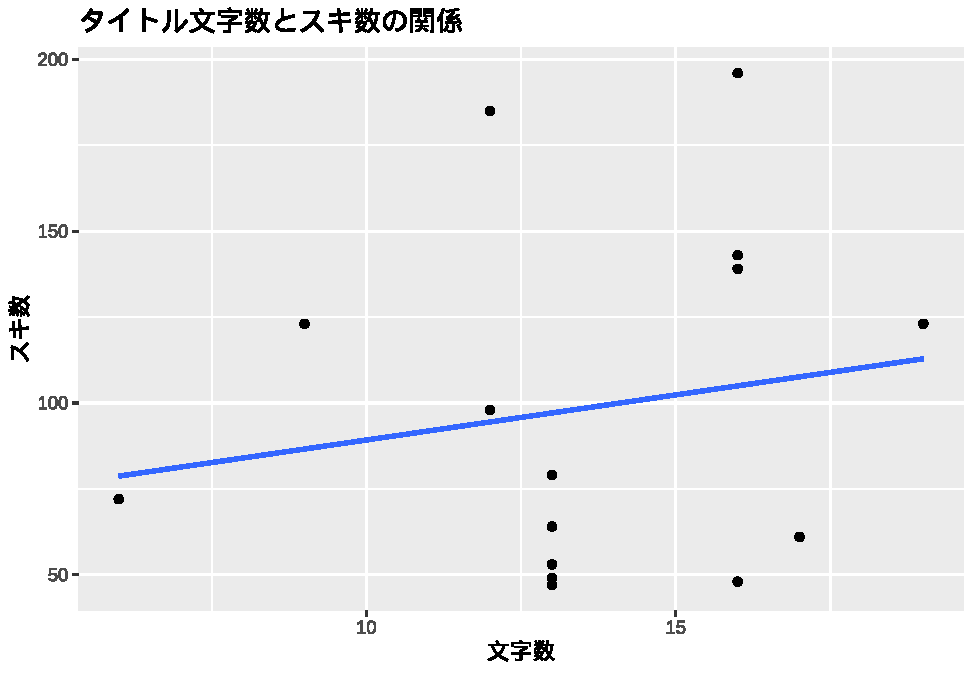
\includegraphics[keepaspectratio]{note-report_files/figure-latex/unnamed-chunk-3-1.pdf}}

\begin{Shaded}
\begin{Highlighting}[]
\DocumentationTok{\#\#投稿時間とスキ数の関係}
\FunctionTok{ggplot}\NormalTok{(note\_data, }\FunctionTok{aes}\NormalTok{(}\AttributeTok{x =}\NormalTok{ time, }\AttributeTok{y =}\NormalTok{ likes)) }\SpecialCharTok{+}
  \FunctionTok{geom\_point}\NormalTok{() }\SpecialCharTok{+}
  \FunctionTok{geom\_smooth}\NormalTok{(}\AttributeTok{method =} \StringTok{"lm"}\NormalTok{, }\AttributeTok{se =} \ConstantTok{FALSE}\NormalTok{) }\SpecialCharTok{+}
  \FunctionTok{labs}\NormalTok{(}\AttributeTok{title =} \StringTok{"投稿時間とスキ数の関係"}\NormalTok{, }\AttributeTok{x =} \StringTok{"投稿時間"}\NormalTok{, }\AttributeTok{y =} \StringTok{"スキ数"}\NormalTok{)}
\end{Highlighting}
\end{Shaded}

\pandocbounded{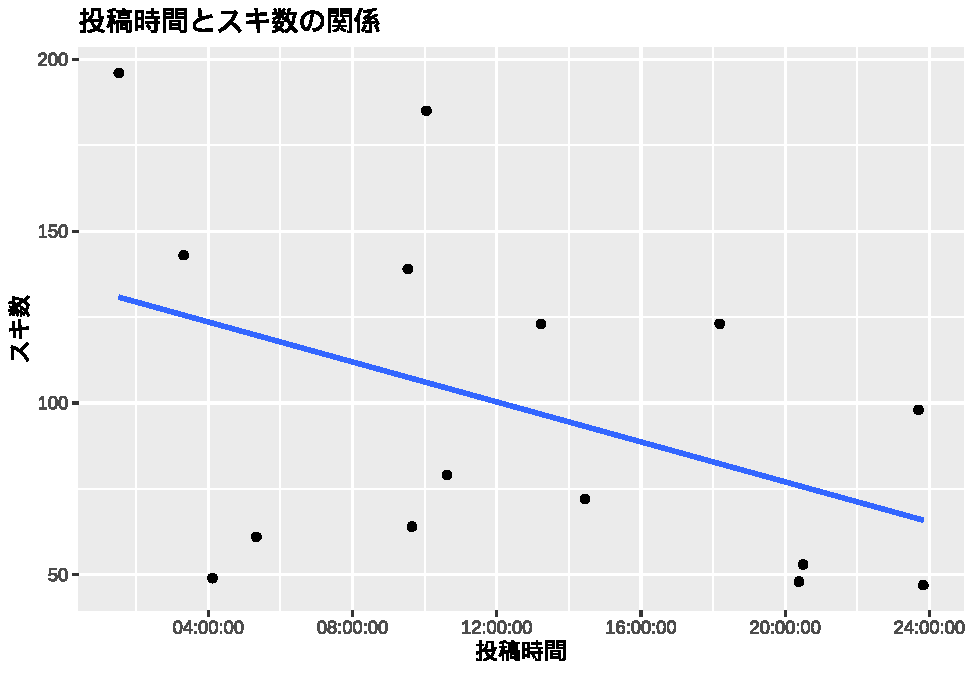
\includegraphics[keepaspectratio]{note-report_files/figure-latex/unnamed-chunk-3-2.pdf}}

\begin{Shaded}
\begin{Highlighting}[]
\DocumentationTok{\#\#文字数とスキ数の関係}
\FunctionTok{ggplot}\NormalTok{(note\_data, }\FunctionTok{aes}\NormalTok{(}\AttributeTok{x =}\NormalTok{ length, }\AttributeTok{y =}\NormalTok{ likes)) }\SpecialCharTok{+}
  \FunctionTok{geom\_point}\NormalTok{() }\SpecialCharTok{+}
  \FunctionTok{geom\_smooth}\NormalTok{(}\AttributeTok{method =} \StringTok{"lm"}\NormalTok{, }\AttributeTok{se =} \ConstantTok{FALSE}\NormalTok{) }\SpecialCharTok{+}
  \FunctionTok{labs}\NormalTok{(}\AttributeTok{title =} \StringTok{"文字数とスキ数の関係"}\NormalTok{, }\AttributeTok{x =} \StringTok{"文字数"}\NormalTok{, }\AttributeTok{y =} \StringTok{"スキ数"}\NormalTok{)}
\end{Highlighting}
\end{Shaded}

\pandocbounded{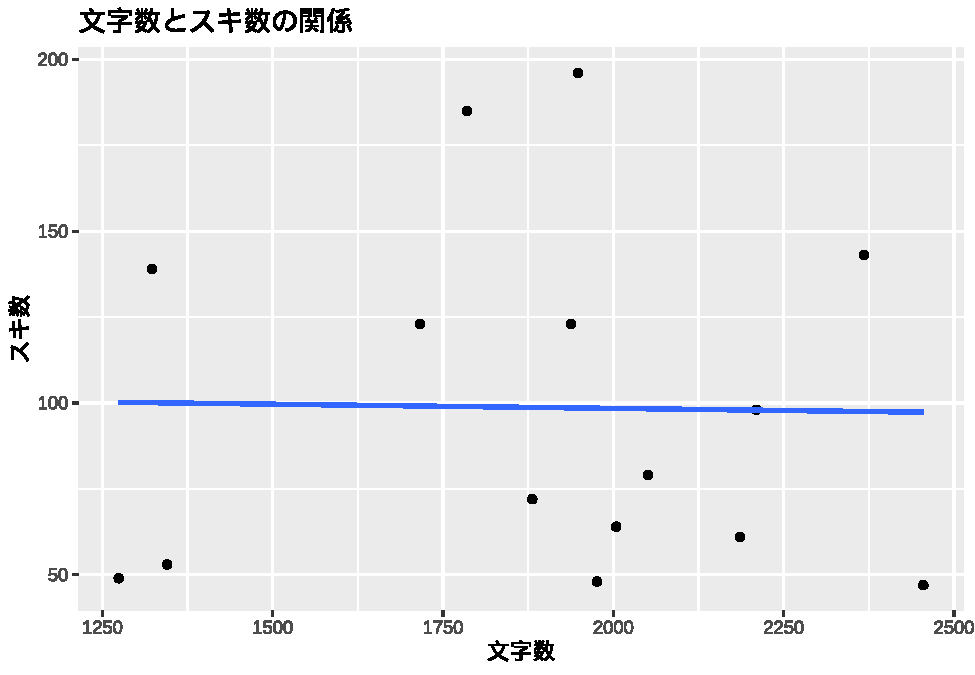
\includegraphics[keepaspectratio]{note-report_files/figure-latex/unnamed-chunk-3-3.pdf}}

\begin{Shaded}
\begin{Highlighting}[]
\DocumentationTok{\#\#タグ別の平均スキ数}
\NormalTok{tag\_summary }\OtherTok{\textless{}{-}}\NormalTok{ note\_data\_long }\SpecialCharTok{\%\textgreater{}\%}
  \FunctionTok{group\_by}\NormalTok{(tag) }\SpecialCharTok{\%\textgreater{}\%}
  \FunctionTok{summarise}\NormalTok{(}\AttributeTok{mean\_like =} \FunctionTok{mean}\NormalTok{(likes), }\AttributeTok{.groups =} \StringTok{"drop"}\NormalTok{)}
\FunctionTok{ggplot}\NormalTok{(tag\_summary, }\FunctionTok{aes}\NormalTok{(}\AttributeTok{x =} \FunctionTok{reorder}\NormalTok{(tag, mean\_like), }\AttributeTok{y =}\NormalTok{ mean\_like)) }\SpecialCharTok{+}
  \FunctionTok{geom\_col}\NormalTok{() }\SpecialCharTok{+}
  \FunctionTok{coord\_flip}\NormalTok{() }\SpecialCharTok{+}
  \FunctionTok{labs}\NormalTok{(}\AttributeTok{title =} \StringTok{"タグ別平均スキ数"}\NormalTok{, }\AttributeTok{x =} \StringTok{"タグ"}\NormalTok{, }\AttributeTok{y =} \StringTok{"平均スキ数"}\NormalTok{)}
\end{Highlighting}
\end{Shaded}

\pandocbounded{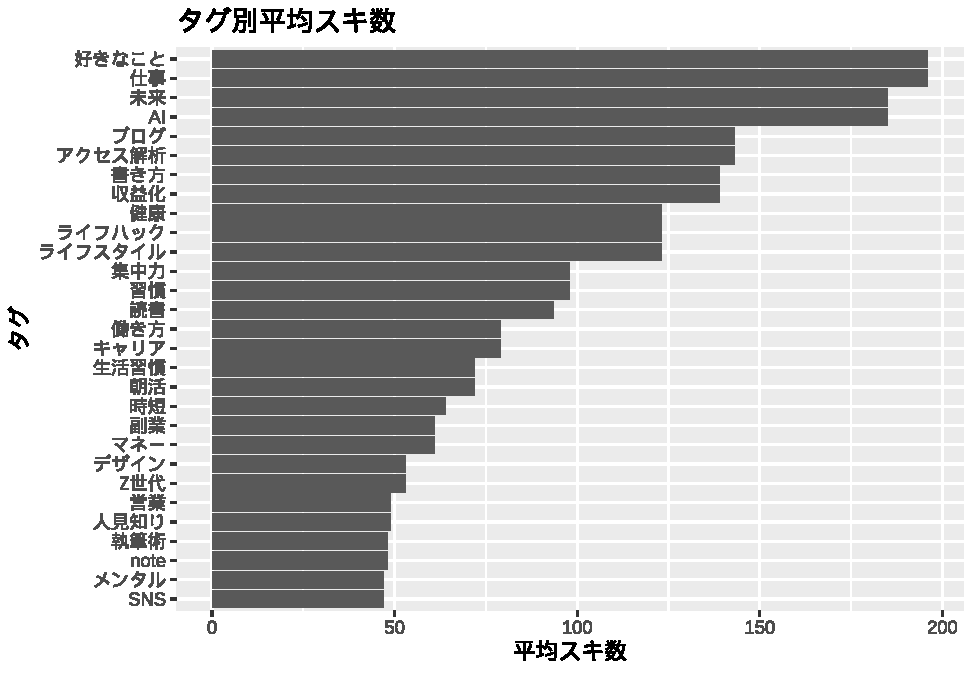
\includegraphics[keepaspectratio]{note-report_files/figure-latex/unnamed-chunk-3-4.pdf}}

\begin{Shaded}
\begin{Highlighting}[]
\DocumentationTok{\#\#スキ数が高い記事の特徴を見る}
\NormalTok{note\_data }\SpecialCharTok{\%\textgreater{}\%}
  \FunctionTok{arrange}\NormalTok{(}\FunctionTok{desc}\NormalTok{(likes)) }\SpecialCharTok{\%\textgreater{}\%}
  \FunctionTok{select}\NormalTok{(title, title\_num, time, length, pv, likes, like\_rate) }\SpecialCharTok{\%\textgreater{}\%}
  \FunctionTok{head}\NormalTok{(}\DecValTok{5}\NormalTok{)}
\end{Highlighting}
\end{Shaded}

\begin{verbatim}
## # A tibble: 5 x 7
##   title                             title_num time  length    pv likes like_rate
##   <chr>                                 <int> <tim>  <dbl> <dbl> <dbl>     <dbl>
## 1 「好き」を仕事にするための第一歩         16 01:31   1948  1369   196    0.143 
## 2 生成AIとの共存を考える                   12 10:03   1785  1142   185    0.162 
## 3 ブログアクセスが3倍になった理由          16 03:19   2368   789   143    0.181 
## 4 noteを使って収益化できるか?             16 09:32   1323   768   139    0.181 
## 5 30代でキャリアに悩んだときに読んだ本~~        19 18:11   1716  1289   123    0.0954
\end{verbatim}

\begin{center}\rule{0.5\linewidth}{0.5pt}\end{center}

\section{データ解析(エンゲージメント:スキ率)}\label{ux30c7ux30fcux30bfux89e3ux6790ux30a8ux30f3ux30b2ux30fcux30b8ux30e1ux30f3ux30c8ux30b9ux30adux7387}

\begin{Shaded}
\begin{Highlighting}[]
\DocumentationTok{\#\#タイトルの文字数とスキ率の関係}
\FunctionTok{ggplot}\NormalTok{(note\_data, }\FunctionTok{aes}\NormalTok{(}\AttributeTok{x =}\NormalTok{ title\_num, }\AttributeTok{y =}\NormalTok{ like\_rate)) }\SpecialCharTok{+}
  \FunctionTok{geom\_point}\NormalTok{() }\SpecialCharTok{+}
  \FunctionTok{geom\_smooth}\NormalTok{(}\AttributeTok{method =} \StringTok{"lm"}\NormalTok{, }\AttributeTok{se =} \ConstantTok{FALSE}\NormalTok{) }\SpecialCharTok{+}
  \FunctionTok{labs}\NormalTok{(}\AttributeTok{title =} \StringTok{"タイトル文字数とスキ率の関係"}\NormalTok{, }\AttributeTok{x =} \StringTok{"文字数"}\NormalTok{, }\AttributeTok{y =} \StringTok{"スキ率"}\NormalTok{)}
\end{Highlighting}
\end{Shaded}

\pandocbounded{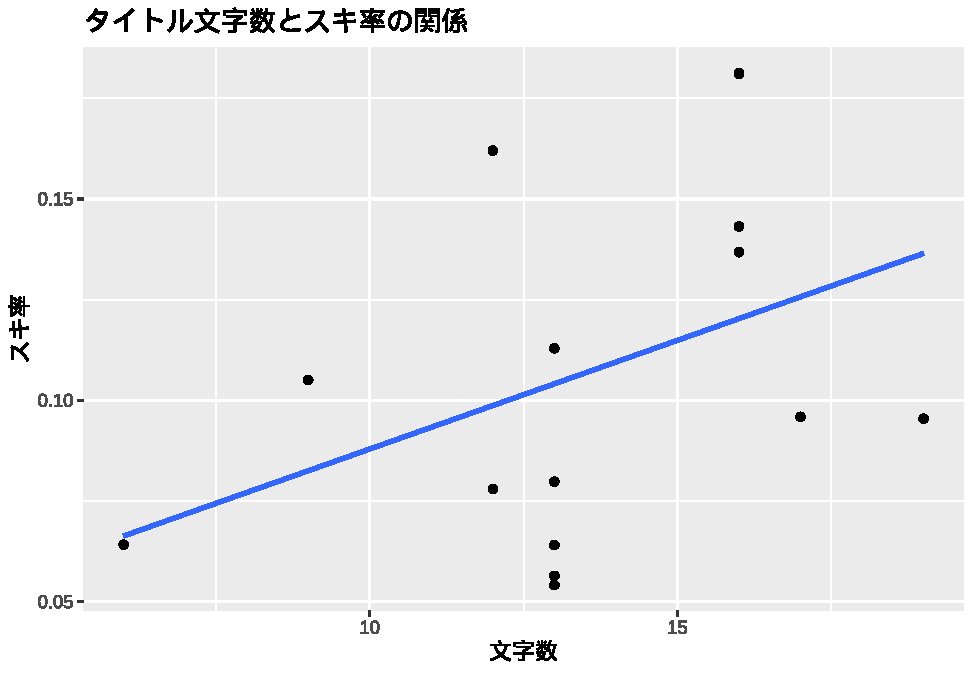
\includegraphics[keepaspectratio]{note-report_files/figure-latex/unnamed-chunk-4-1.pdf}}

\begin{Shaded}
\begin{Highlighting}[]
\DocumentationTok{\#\#タイトルの文字数とスキ率との相関関係}
\FunctionTok{cor}\NormalTok{(note\_data}\SpecialCharTok{$}\NormalTok{title\_num, note\_data}\SpecialCharTok{$}\NormalTok{like\_rate)}
\end{Highlighting}
\end{Shaded}

\begin{verbatim}
## [1] 0.4008658
\end{verbatim}

\begin{Shaded}
\begin{Highlighting}[]
\DocumentationTok{\#\#投稿時間とスキ率の関係}
\FunctionTok{ggplot}\NormalTok{(note\_data, }\FunctionTok{aes}\NormalTok{(}\AttributeTok{x =}\NormalTok{ time, }\AttributeTok{y =}\NormalTok{ like\_rate)) }\SpecialCharTok{+}
  \FunctionTok{geom\_point}\NormalTok{() }\SpecialCharTok{+}
  \FunctionTok{geom\_smooth}\NormalTok{(}\AttributeTok{method =} \StringTok{"lm"}\NormalTok{, }\AttributeTok{se =} \ConstantTok{FALSE}\NormalTok{) }\SpecialCharTok{+}
  \FunctionTok{labs}\NormalTok{(}\AttributeTok{title =} \StringTok{"投稿時間とスキ率の関係"}\NormalTok{, }\AttributeTok{x =} \StringTok{"投稿時間"}\NormalTok{, }\AttributeTok{y =} \StringTok{"スキ率"}\NormalTok{)}
\end{Highlighting}
\end{Shaded}

\pandocbounded{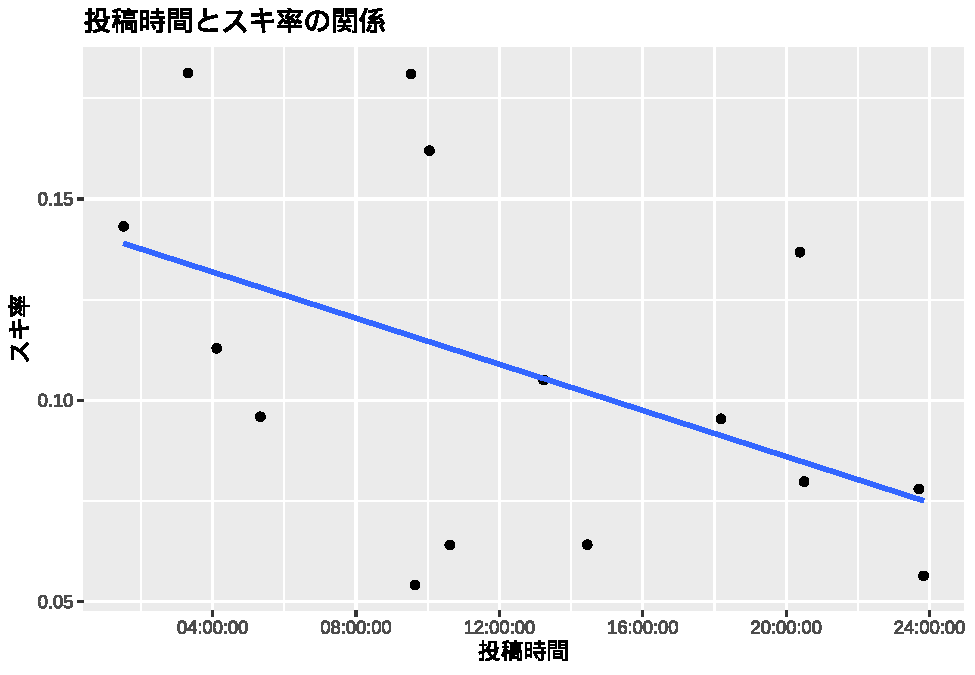
\includegraphics[keepaspectratio]{note-report_files/figure-latex/unnamed-chunk-4-2.pdf}}

\begin{Shaded}
\begin{Highlighting}[]
\DocumentationTok{\#\#投稿時間帯とスキ率の関係}
\FunctionTok{ggplot}\NormalTok{(note\_data, }\FunctionTok{aes}\NormalTok{(}\AttributeTok{x =}\NormalTok{ time\_category, }\AttributeTok{y =}\NormalTok{ like\_rate)) }\SpecialCharTok{+}
  \FunctionTok{geom\_boxplot}\NormalTok{() }\SpecialCharTok{+}
  \FunctionTok{labs}\NormalTok{(}\AttributeTok{title =} \StringTok{"時間帯別のスキ率"}\NormalTok{, }\AttributeTok{x =} \StringTok{"時間帯"}\NormalTok{, }\AttributeTok{y =} \StringTok{"スキ率"}\NormalTok{)}
\end{Highlighting}
\end{Shaded}

\pandocbounded{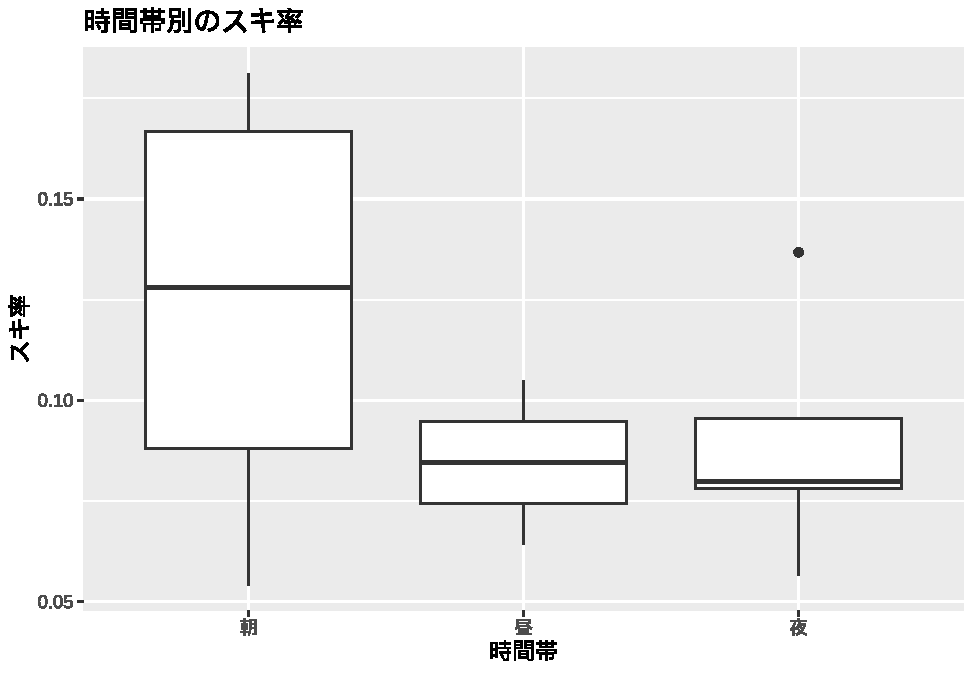
\includegraphics[keepaspectratio]{note-report_files/figure-latex/unnamed-chunk-4-3.pdf}}

\begin{Shaded}
\begin{Highlighting}[]
\DocumentationTok{\#\#文字数とスキ率の関係}
\FunctionTok{ggplot}\NormalTok{(note\_data, }\FunctionTok{aes}\NormalTok{(}\AttributeTok{x =}\NormalTok{ length, }\AttributeTok{y =}\NormalTok{ like\_rate)) }\SpecialCharTok{+}
  \FunctionTok{geom\_point}\NormalTok{() }\SpecialCharTok{+}
  \FunctionTok{geom\_smooth}\NormalTok{(}\AttributeTok{method =} \StringTok{"lm"}\NormalTok{, }\AttributeTok{se =} \ConstantTok{FALSE}\NormalTok{) }\SpecialCharTok{+}
  \FunctionTok{labs}\NormalTok{(}\AttributeTok{title =} \StringTok{"文字数とスキ率の関係"}\NormalTok{, }\AttributeTok{x =} \StringTok{"文字数"}\NormalTok{, }\AttributeTok{y =} \StringTok{"スキ率"}\NormalTok{)}
\end{Highlighting}
\end{Shaded}

\pandocbounded{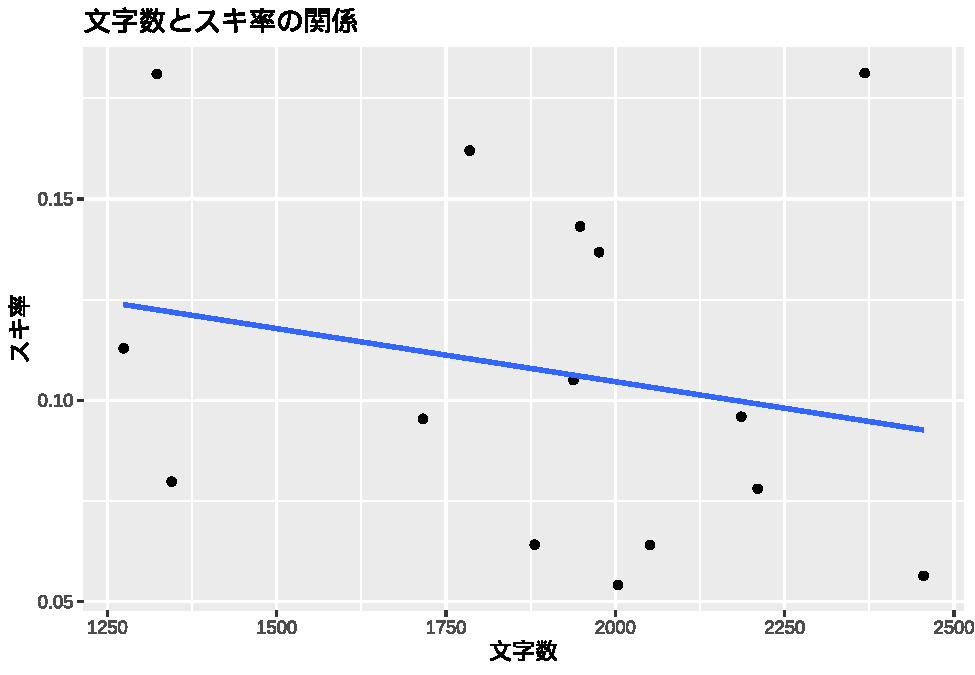
\includegraphics[keepaspectratio]{note-report_files/figure-latex/unnamed-chunk-4-4.pdf}}

\begin{Shaded}
\begin{Highlighting}[]
\DocumentationTok{\#\#タグ別の平均スキ率}
\NormalTok{tag\_summary }\OtherTok{\textless{}{-}}\NormalTok{ note\_data\_long }\SpecialCharTok{\%\textgreater{}\%}
  \FunctionTok{group\_by}\NormalTok{(tag) }\SpecialCharTok{\%\textgreater{}\%}
  \FunctionTok{summarise}\NormalTok{(}\AttributeTok{mean\_like\_rate =} \FunctionTok{mean}\NormalTok{(like\_rate), }\AttributeTok{.groups =} \StringTok{"drop"}\NormalTok{)}
\FunctionTok{ggplot}\NormalTok{(tag\_summary, }\FunctionTok{aes}\NormalTok{(}\AttributeTok{x =} \FunctionTok{reorder}\NormalTok{(tag, mean\_like\_rate), }\AttributeTok{y =}\NormalTok{ mean\_like\_rate)) }\SpecialCharTok{+}
  \FunctionTok{geom\_col}\NormalTok{() }\SpecialCharTok{+}
  \FunctionTok{coord\_flip}\NormalTok{() }\SpecialCharTok{+}
  \FunctionTok{labs}\NormalTok{(}\AttributeTok{title =} \StringTok{"タグ別平均スキ率"}\NormalTok{, }\AttributeTok{x =} \StringTok{"タグ"}\NormalTok{, }\AttributeTok{y =} \StringTok{"平均スキ率"}\NormalTok{)}
\end{Highlighting}
\end{Shaded}

\pandocbounded{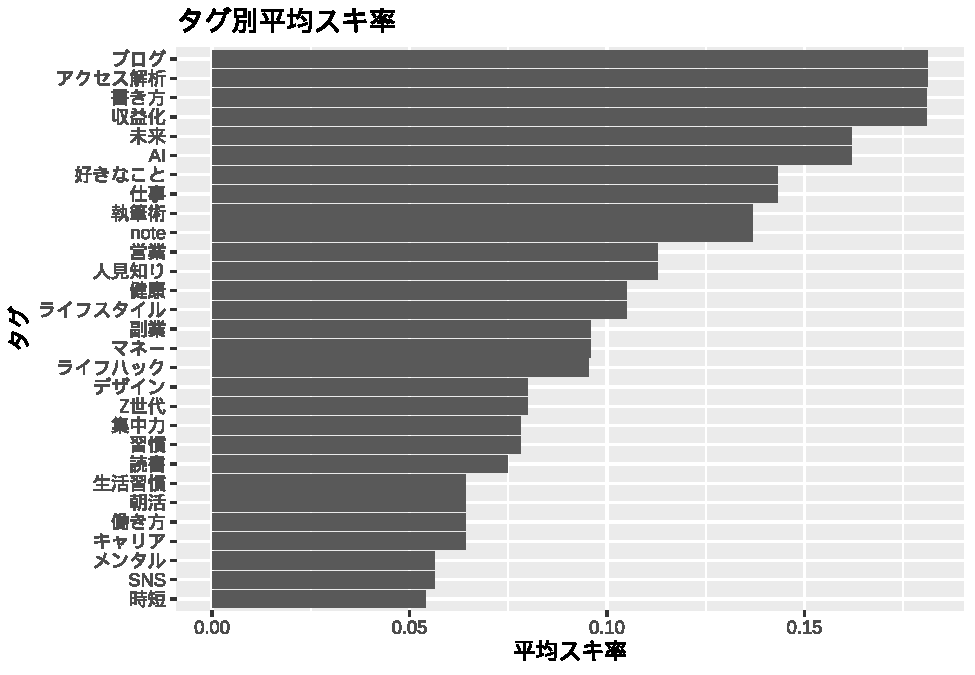
\includegraphics[keepaspectratio]{note-report_files/figure-latex/unnamed-chunk-4-5.pdf}}

\begin{Shaded}
\begin{Highlighting}[]
\DocumentationTok{\#\#スキ率が高い記事の特徴を見る}
\NormalTok{note\_data }\SpecialCharTok{\%\textgreater{}\%}
  \FunctionTok{arrange}\NormalTok{(}\FunctionTok{desc}\NormalTok{(like\_rate)) }\SpecialCharTok{\%\textgreater{}\%}
  \FunctionTok{select}\NormalTok{(title, title\_num, time, length, pv, likes, like\_rate) }\SpecialCharTok{\%\textgreater{}\%}
  \FunctionTok{head}\NormalTok{(}\DecValTok{5}\NormalTok{)}
\end{Highlighting}
\end{Shaded}

\begin{verbatim}
## # A tibble: 5 x 7
##   title                            title_num time   length    pv likes like_rate
##   <chr>                                <int> <time>  <dbl> <dbl> <dbl>     <dbl>
## 1 ブログアクセスが3倍になった理由         16 03:19    2368   789   143     0.181
## 2 noteを使って収益化できるか?            16 09:32    1323   768   139     0.181
## 3 生成AIとの共存を考える                  12 10:03    1785  1142   185     0.162
## 4 「好き」を仕事にするための第一歩        16 01:31    1948  1369   196     0.143
## 5 書くことがない日のnote活用術            16 20:23    1976   351    48     0.137
\end{verbatim}

\begin{longtable}[]{@{}
  >{\raggedright\arraybackslash}p{(\linewidth - 0\tabcolsep) * \real{1.0000}}@{}}
\toprule\noalign{}
\endhead
\bottomrule\noalign{}
\endlastfoot
\# 考察・まとめ \\
- 昼に投稿すると安定してよく閲覧されることがわかった。 -
「好きなこと」「仕事」などのタグが高閲覧数に貢献していた。 -
閲覧数が多いとスキと好評価をもらいやすい傾向にあった。 -
昼の投稿は閲覧されやすいが、好評価はされにくいことがわかった。 -
「好きなこと」「仕事」などのタグが閲覧数と同じようにスキに貢献していたが、閲覧されば好評価を受けやすいのは「ブログ」「アクセス解析」「書き方」「収益化」など実益に繋がりそうなタグがついた記事であった。 \\
今後、投稿内容やタグに合わせて投稿時間を工夫することで、さらに多くのユーザーに読まれる可能性がある。 \\
\end{longtable}

\section{参考情報}\label{ux53c2ux8003ux60c5ux5831}

\begin{itemize}
\tightlist
\item
  仮想データ:step01\_note\_virtual\_data.csv
\item
  使用言語:R(tidyverse, readr, knitr, kableExtra, dplyr, tidyr,
  stringr, showtext, gridExtra, grid)
\end{itemize}

\end{document}
